\documentclass[tikz,border=2pt]{standalone}
\usepackage{amsmath,amssymb}
\usepackage{pgfplots}
\pgfplotsset{compat=1.18}
\usetikzlibrary{arrows.meta}

\begin{document}
% f(x) = x^2 - x on [a, b] = [-1, 2]: f(a) = f(b) = 2, and f'(c) = 0 at c = 1/2, f(c) = -1/4.
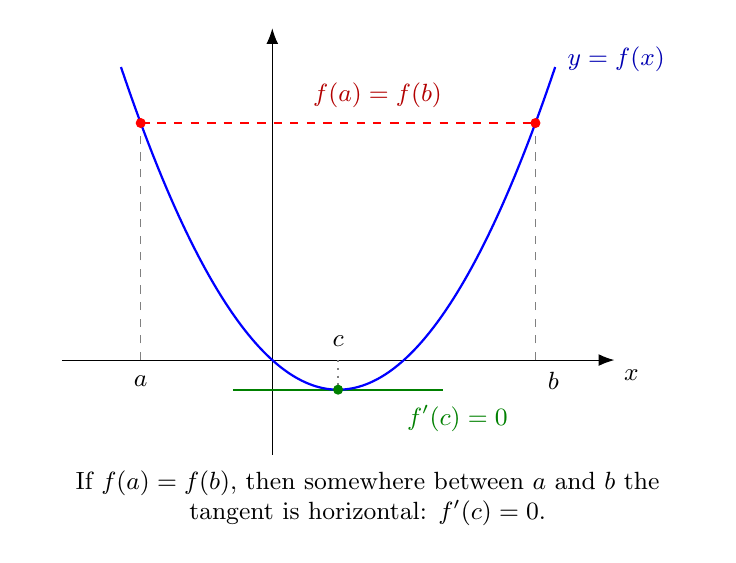
\begin{tikzpicture}[every node/.style={font=\small}]
	\begin{axis}[
		width=8.6cm, height=7cm,
		axis lines=middle, axis line style={-{Latex[length=2mm]}},
		xmin=-1.6, xmax=2.6, ymin=-0.8, ymax=2.8,
		xtick=\empty, ytick=\empty,
		xlabel={$x$}, xlabel style={below right},
		samples=150, clip=false
		]
		\addplot[gray, dashed] coordinates {(-1,0) (-1,2)};
		\addplot[gray, dashed] coordinates {(2,0) (2,2)};
		\addplot[gray, dotted, thick] coordinates {(0.5,0) (0.5,-0.25)};
		\addplot[red, dashed, thick, domain=-1:2] {2};
		\addplot[green!50!black, thick, domain=-0.3:1.3] {-0.25};
		\addplot[blue, thick, domain=-1.15:2.15] {x^2-x};
		\addplot[only marks, mark=*, mark size=1.6pt, red] coordinates {(-1,2) (2,2)};
		\addplot[only marks, mark=*, mark size=1.6pt, green!50!black] coordinates {(0.5,-0.25)};
		\node[anchor=north, font=\small] at (axis cs:-1,-0.05) {$a$};
		\node[anchor=north west, font=\small] at (axis cs:2.02,-0.02) {$b$};
		\node[anchor=south, font=\small] at (axis cs:0.5,0.03) {$c$};
		\node[red!70!black, anchor=south] at (axis cs:0.8,2.05) {$f(a)=f(b)$};
		\node[green!50!black, anchor=north west] at (axis cs:0.95,-0.3) {$f'(c)=0$};
		\node[blue!70!black, anchor=west] at (axis cs:2.17,{2.17^2-2.17}) {$y=f(x)$};
	\end{axis}
	\node[anchor=north, align=flush center, text width=8.4cm] at ([yshift=-2pt]current bounding box.south) {If $f(a)=f(b)$, then somewhere between $a$ and $b$ the tangent is horizontal: $f'(c)=0$.};
\end{tikzpicture}
\end{document}
